\chapter{Gegenmassnahmen}
\label{ch:Gegenmassnahmen}

An dieser Stelle ist es wichtig Schemen zu finden, die resistent gegen ASAs sind. Aus den Angriffen, die ich zuvor vorgestellt habe können wir lernen, dass wir Schemen nutzen sollten, die deterministisch und stateful sind. Vor allem stateless Schemen haben sich als gefährdet erwiesen, da Angriffe bei diesen besonders schwer zu entdecken sind. Wichtig hierbei ist, dass eigentliche Sicherheitseigenschaften wie Vertraulichkeit und Authentizität keinen Einfluss auf die Resistenz gegen ASAs bieten. Diese Resistenz wird nur in einer Klasse von symmetrischen Schemen sichergestellt, einer Klasse die von den Autoren unique ciphertext schemes genannt wird.

\begin{figure}[!ht]
	\centering
	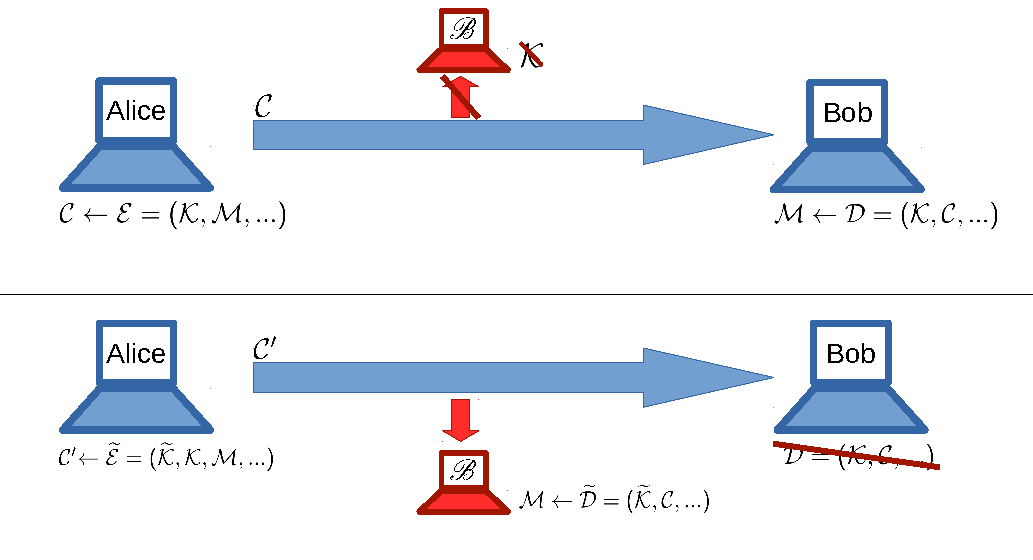
\includegraphics[width=\textwidth]{image/unique}
	\caption{unique chiphertext scheme.}
	\label{fig:unique}
\end{figure}

Um ein unique ciphertext Schema zu definieren, nehmen wir an, in dem symmetrischen Verschlüsselungsschema $\Pi = (\mathcal{K}, \mathcal{E}, \mathcal{D})$ soll folgendes gelten: Für jedes Tupel $(\mathcal{K}$, $\mathcal{M}, \mathcal{A}, \sigma$) gibt es höchstens ein $\mathcal{C}$, das entschlüsselt die Nachricht $\mathcal{M}$ unter $\mathcal{K}$ ergibt. Also wenn diese Abbildung injektiv ist (siehe \ref{fig:injektiv}), dann ist $\Pi$ ein unique ciphertext scheme.

\begin{figure}[!ht]
	\centering
	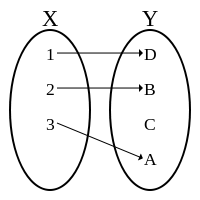
\includegraphics[width=0.3\textwidth]{image/Injection}
	\caption{Injektivität.}
	\label{fig:injektiv}
\end{figure}

Diese Eigenschaft trifft keineswegs auf alle Schemen zu. Für zwei verschiedene Chiffretexte $\mathcal{C} \neq \mathcal{C}^{'}$ muss also immer $\mathcal{D}(\mathcal{C}) \neq \mathcal{D}(\mathcal{C}^{'})$ gelten. Aus dieser Eigenschaft können wir Theorem \ref{theo:unique} erstellen. Wie in Abbildung \ref{fig:unique} zu sehen, sorgt eine Subversion von $\Pi$ dafür, dass ein Chiffretext $\mathcal{C}^{'} \neq \mathcal{C}$ beim Entschlüsseln bei Bob zu einer nicht korrekten Nachricht führt, also das Schema die Korrektheit aus Abschnitt \ref{sec:korrekt} nicht erfüllt. In diesem Fall würde die Subversion entdeckt werden.
	
\begin{theorem}
\label{theo:unique}

Sei $\Pi = (K, E, D)$ ein unique ciphertext scheme, dann gibt es kein Subversion $\widetilde{\Pi} = (\widetilde{K}, \widetilde{E}, \widetilde{D})$ von $\Pi$, mit der korrekt mit $\mathcal{D}$ entschlüsselt werden kann und $\mathscr{B}$ hat keine Erfolgschancen gegen $\Pi$.

\end{theorem}
